\section*{Closed Path}

If the initial and terminal points of a path are identical, then the path is called a \textbf{closed path}.

\vspace{0.5em}
\noindent \textbf{Examples of Closed Paths:}
\begin{itemize}
    \item A circle or ellipse returning to its starting point.
\end{itemize}

\section*{ Non-Closed Path}

If the initial and terminal points of a path are not identical, then the path is called a \textbf{non-closed path} (or open path).

\vspace{0.5em}
\noindent \textbf{Example of a Non-Closed Path:}
\begin{itemize}
    \item An open curve or line segment where the start and end points do not coincide.
\end{itemize}
\section*{Periodic Solution}

Consider the dynamical system:
\begin{equation}
    \begin{aligned}
        \dot{x} &= P(x, y) \\
        \dot{y} &= Q(x, y)
    \end{aligned} \sidenote{1}
\end{equation}

\noindent Let $x = f(t)$ and $y = g(t)$ be a solution of system (1). Then the solution is called a \textbf{periodic solution} if there exists a constant $T > 0$ such that:
\[
f(t + T) = f(t) \quad \text{and} \quad g(t + T) = g(t) \quad \text{for all } t
\]

\noindent Here, $T$ is called the \textbf{period} of the solution.
\section*{Limit Cycle}

A closed path $C$ of a system:
\begin{equation}
    \begin{aligned}
        \dot{x} &= P(x, y) \\
        \dot{y} &= Q(x, y)
    \end{aligned} \sidenote{1}
\end{equation}

\noindent which is approached spirally from either inside or outside by a non-closed path $C_1$ of system (1) as $t \to +\infty$ or $t \to -\infty$ is called a \textbf{limit cycle} of the system (1).
\begin{center}
    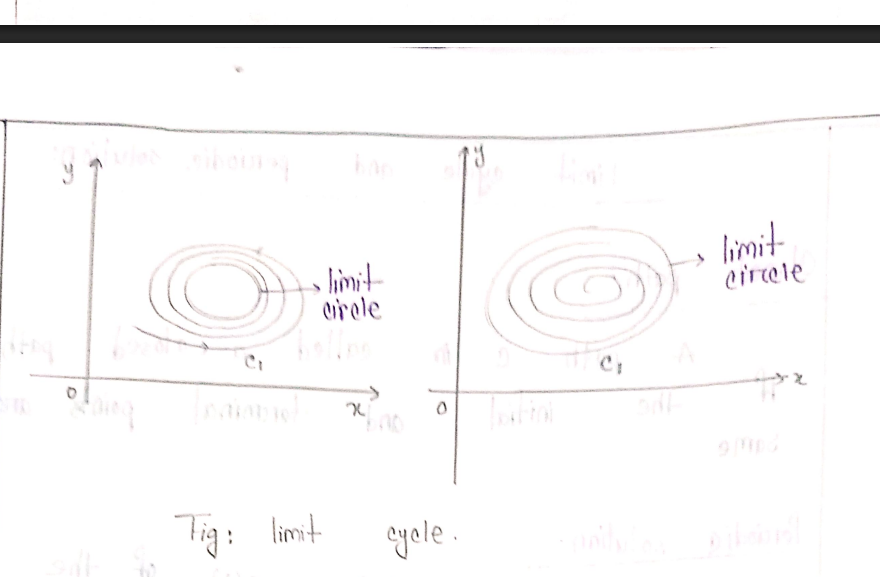
\includegraphics[width=0.5 \textwidth]{Image/limit cycle.png}
\end{center}